%% 
% @file  GNE-howto.Rnw
% @brief sweave file for the vignette
%
% @author Christophe Dutang
%
%


\documentclass[11pt, a4paper]{article}

%\VignetteIndexEntry{User guide for the GNE package}
%\VignettePackage{GNE}
%\VignetteKeyword{nonlinear}

  
% package

%American Mathematical Society (AMS) math symbols
\usepackage{amsfonts,amssymb,amsmath}
%english typography
\usepackage[english]{babel}
\usepackage{a4wide,courier,newlfont}

% 8 bit accents 
%\usepackage[applemac]{inputenc} %MAC encoding
\usepackage[utf8]{inputenc} %UNIX encoding
%\usepackage[ansinew]{inputenc} %WINDOWS encoding

%graph
\usepackage[dvips]{graphicx}
\usepackage{color,graphics, subfig}

%citation
\usepackage{natbib}

%text style
\usepackage{ulem}

%reference hypertext
\usepackage[hyperfootnotes=false]{hyperref}

%footnote
\usepackage[stable]{footmisc}
\usepackage{perpage}
\MakePerPage[1]{footnote}

%multicol package
\usepackage{multirow, multicol}

%url
\usepackage{url}

%header
\pagestyle{headings}


% layout
\normalsize\setlength{\parskip}{\baselineskip}
\setlength{\oddsidemargin}{25mm}
\setlength{\evensidemargin}{25mm}
\setlength{\voffset}{-2.54cm}
\setlength{\hoffset}{-3.8cm}
\setlength{\textwidth}{180mm}
\setlength{\topmargin}{0mm}
\setlength{\headheight}{15mm}
\setlength{\headsep}{11mm}
\setlength{\topskip}{0mm}
\setlength{\textheight}{230mm}

% macros
\newcommand{\HRule}{\noindent\rule{\linewidth}{1pt}}
\newcommand{\II}{\mbox{\large 1\hskip -0,353em 1}}
\newcommand{\abs}[1]{\lvert#1\rvert}
\newcommand{\norm}[1]{\lVert#1\rVert}
\newcommand{\ligne}{\rule[2mm]{.3\textwidth}{0,5mm}\\}
\newcommand{\pkg}{\textbf}
\newcommand{\sigle}{\textsc}
\newcommand{\code}{\texttt}
\newcommand{\soft}{\textsf}
\newcommand{\myskip}{\vspace{\parskip}}
\newcommand{\txtm}[1]{\textrm{~~#1~~}}
\newcommand{\expo}{\textsuperscript}
\newcommand{\ind}{1\!\!1}
\newcommand{\mat}[1]{\mathbf{#1}}
\newcommand{\blank}{ \clearpage{\pagestyle{empty}\cleardoublepage} }
\newcommand{\card}{\textrm{Card}}
\newcommand{\diag}{\textrm{diag}}
\newcommand{\NIF}{\textrm{NIF}}
\newcommand{\GAP}{\textrm{GAP}}
\newcommand{\Jac}{\textrm{Jac\hskip+.1em}}
\newcommand{\R}{\ensuremath{\mathbb{R}}}


% footnote in table or legend
\newcounter{noteTabCap} 
\newcommand{\initFmark}{\setcounter{noteTabCap}{0}} %init noteTabCap counter
\newcommand{\fmark}{\footnotemark  \addtocounter{noteTabCap}{1}} %mark footnote
\newcommand{\updateFtext}{\addtocounter{footnote}{-\value{noteTabCap}}} %update footnote counter
\newcommand{\ftext}[1]{\addtocounter{footnote}{1}  \footnotetext{#1}} %set the footnote text

%theorems
\newtheorem{mydef}{Definition}



\title{User guide for the \pkg{GNE} package}


\author{Christophe Dutang}


\usepackage{Sweave}
\begin{document}
\Sconcordance{concordance:GNE-howto.tex:GNE-howto.Rnw:%
1 103 1 1 0 7 1 1 2 4 0 1 2 141 1 1 2 1 0 1 1 1 8 7 0 1 2 1 3 2 0 1 3 5 %
0 1 2 19 1 1 12 11 0 1 2 4 0 1 2 5 1 1 2 1 0 1 1 1 4 14 0 1 2 2 1 1 6 5 %
0 3 1 10 0 1 2 167 1 1 2 1 0 1 2 11 0 1 2 2 1 1 3 11 0 1 2 11 0 1 2 144 %
1 1 2 1 0 1 3 13 0 1 2 132 1 1 4 3 0 1 3 2 0 1 3 2 0 1 2 1 4 12 0 1 5 %
13 0 1 2 610 1}


\maketitle


As usual, the \pkg{GNE} package is loaded via the \code{library} function. In the following, we assume that the line below has been called
%%% R code
\begin{Schunk}
\begin{Sinput}
> library(GNE)
\end{Sinput}
\end{Schunk}
%%%

%________________________________________________________________________
\section{Introduction}
%________________________________________________________________________

\begin{mydef}[GNEP]
We define the generalized Nash equilibrium problem GNEP($N, \theta_i, X_i$) as the solutions $x^\star$ of the $N$ sub-problems
$$
\forall i = 1, \dots, N, x_i^\star \txtm{solves} 
\underset{ y_i }{\min} 
\quad
\theta_i(y_i, x_{-i}^\star)
\txtm{such that} x_i^\star \in X_i(x_{-i}^\star),
$$
where $X_i(x_{-i})$ is the action space of player $i$ given others player actions $x_{-i}$.
\end{mydef}

If we have parametrized action space $X_i(x_{-i}) = \{ y_i, g_i(y_i, x_{-i}) \leq 0  \}$, we denote the GNEP by  GNEP($N, \theta_i, g_i$).

We denote by $X(x) $ the action set $X(x) = X_1(x_{-1}) \times \dots \times X_N(x_{-N})$. For standard NE, this set does not depend on $x$.

The following example seems very basic, but in fact it has particular features, one of them is to have four solutions, i.e. four GNEs.
Let $N=2$. The objective functions are defined as
$$
\theta_1(x) = (x_1-2)^2 (x_2-4)^4 \txtm{and} \theta_2(x) = (x_2-3)^2 (x_1)^4,
$$
for $x\in \R^2$, while the constraint functions are given by
$$
g_1(x) = x_1+x_2-1 \leq 0 \txtm{and} g_2(x) = 2x_1+x_2-2 \leq 0.
$$
Objective functions can be rewritten as $\theta_i(x) = (x_i - c_i)^2 (x_{-i} d_i)^4$, with $c = (2, 3)$ and
$d=(4,0)$.
First-order derivatives are 
$$
\nabla_j \theta_i(x) = 2 (x_i - c_i) (x_{-i} d_i)^4 \delta_{ij} +  4(x_i - c_i)^2 (x_{-i} d_i)^3 (1- \delta_{ij}),
$$
and
$$
\nabla_j g_1(x) = 1
\txtm{and}
\nabla_j g_2(x) = 2 \delta_{j1} + \delta_{j2}.
$$
Second-order derivatives are
\begin{equation*}
\begin{split}
\nabla_k \nabla_j \theta_i(x) = 2 (x_{-i} d_i)^4 \delta_{ij} \delta_{ik}  
+ 8 (x_i - c_i) (x_{-i} d_i)^3 \delta_{ij} (1-\delta_{ik}) \\
+ 8(x_i - c_i) (x_{-i} d_i)^3 (1- \delta_{ij})  \delta_{ik} 
+ 12(x_i - c_i)^2 (x_{-i} d_i)^2 (1- \delta_{ij})(1- \delta_{ik} ),
\end{split}
\end{equation*}
and
$$
\nabla_k \nabla_j g_1(x) =  \nabla_k \nabla_j g_2(x) = 0.
$$


%________________________________________________________________________
\section{GNEP as a nonsmooth equation}
%________________________________________________________________________


\subsection{Notation and definitions}



From \cite{facchfischpic09}, 
assuming differentiability and a constraint qualification hold, the first-order necessary conditions of player $i$'s subproblem state there exists a Lagrangian multiplier
 $\lambda^i \in  \R^{m_i} $ such that 
\begin{equation*}
\begin{split}
\nabla_{x_i} \theta_{i}(x^\star)   + \sum_{ 1 \leq j \leq m_i } \lambda_{j}^{i\star} \nabla_{x_i} g_{j}^i(x^\star) = &~0~~~~~~~ ( \in \R^{n_i} ). \\
0 \leq \lambda^{i\star},~  - g^i(x^\star) \geq 0,~  g^i(x^\star)^T\lambda^{i\star}= & ~0~~~~~~~ ( \in \R^{m_i} ) .
\end{split}
\end{equation*}
Regrouping the $N$ subproblems, we get the following system.




\begin{mydef}[eKKT]
For the $N$ optimization subproblems for the functions $\theta_i: \R^{n} \mapsto \R$, with constraints $g_i: \R^{n} \mapsto \R^{m_i}$, the KKT conditions can be regrouped such that
there exists $\lambda \in \R^m$ and 
$$
\tilde L(x, \lambda) = 0 \txtm{and} 0 \leq \lambda \perp  G(x) \leq  0,
$$
where $L$ and $G$ are given by
$$
\tilde L(x, \lambda) = 
\left( 
\begin{matrix}
\nabla_{x_1} \theta_1(x) + \Jac g^{1}(x)^T \lambda^1 \\
\vdots \\
\nabla_{x_N} \theta_ N(x) + \Jac g^{N}(x)^T \lambda^N \\
\end{matrix}
\right)  
\in \R^{n}
\txtm{and}
G(x) = 
\left( 
\begin{matrix}
g^1(x) \\
\vdots \\
g^N(x) \\
\end{matrix}
\right) 
\in \R^{m},
$$
with $\Jac g_{i}(x)^T \lambda_i = \sum_{ 1 \leq j \leq m_i } \lambda_{j}^i \nabla_{x_i} g_{j}^i(x)  $. The extended KKT system is denoted by eKKT($N, \theta_i, g_i$).
\end{mydef}

Using complementarity function $\phi(a,b)$ (e.g. $\min(a,b)$), we get the following nonsmooth equation
$$
\Phi(z) = 
\left( 
\begin{matrix}
\tilde L(x, \lambda) \\
\phi_.(-G(x), \lambda) \\
\end{matrix}
\right) = 0 ,
$$
where $\phi_.$ is the component-wise version of the function $\phi$ and $\tilde L$ is the Lagrangian function of the extended system.
The generalized Jacobian is given in Appendix \ref{app:nseq:gencase}.

\subsection{A classic example}

Returning to our example, we define the $\Phi$ as
$$
\Phi(x) = 
\left( 
\begin{matrix}
2(x_1-2) (x_2-4)^4 + \lambda_1 \\
2(x_2-3) (x_1)^4 + \lambda_2 \\
\phi(\lambda_1, 1-  x_1-x_2) \\
\phi(\lambda_2,  2- 2x_1-x_2) \\
\end{matrix}
\right) ,
$$
where $\phi$ denotes a complementarity function.
In \soft{R}, we use 
%%% R code
\begin{Schunk}
\begin{Sinput}
> myarg <- list(C=c(2, 3), D=c(4,0))
> dimx <- c(1, 1)
> #Gr_x_j O_i(x)
> grobj <- function(x, i, j, arg)
+ {
+ 	dij <- 1*(i == j)
+ 	other <- ifelse(i == 1, 2, 1)
+ 	res <- 2*(x[i] - arg$C[i])*(x[other] - arg$D[i])^4*dij 
+ 	res + 4*(x[i] - arg$C[i])^2*(x[other] - arg$D[i])^3*(1-dij) 
+ }
> dimlam <- c(1, 1)
> #g_i(x)
> g <- function(x, i)
+ 	ifelse(i == 1, sum(x[1:2]) - 1, 2*x[1]+x[2]-2)
> #Gr_x_j g_i(x)
> grg <- function(x, i, j)
+ 	ifelse(i == 1, 1, 1 + 1*(i == j))
\end{Sinput}
\end{Schunk}
%%%
Note that the triple dot arguments $\dots$ is used to pass arguments to the complementarity function.

Elements of the generalized Jacobian of $\Phi$ have the following form
$$
\partial \Phi(x) = 
\left\{
\left( 
\begin{matrix}
2(x_2-4)^4 		& 8(x_1-2) (x_2-4)^3  & 1 & 0 \\
8(x_2-3) (x_1)^3  	& 2(x_1)^4 & 0 & 1 \\
-\phi_b'(\lambda_1, 1-  x_1-x_2) & -\phi_b'(\lambda_1, 1-  x_1-x_2)  & \phi_a'(\lambda_1, 1-  x_1-x_2)  & 0 \\
-2\phi_b'(\lambda_2,  2- 2x_1-x_2) & - \phi_b'(\lambda_2,  2- 2x_1-x_2) & 0 & \phi_a'(\lambda_2,  2- 2x_1-x_2) \\
\end{matrix}
\right) 
\right\} ,
$$
where $\phi_a'$ and $\phi_b'$ denote elements of the generalized gradient of the complementarity function.
The corresponding \soft{R} code is 
%%% R code
\begin{Schunk}
\begin{Sinput}
> #Gr_x_k Gr_x_j O_i(x)
> heobj <- function(x, i, j, k, arg)
+ {
+ 	dij <- 1*(i == j)
+ 	dik <- 1*(i == k)
+ 	other <- ifelse(i == 1, 2, 1)
+ 	res <- 2*(x[other] - arg$D[i])^4*dij*dik 
+ 	res <- res + 8*(x[i] - arg$C[i])*(x[other] - arg$D[i])^3*dij*(1-dik)
+ 	res <- res + 8*(x[i] - arg$C[i])*(x[other] - arg$D[i])^3*(1-dij)*dik
+ 	res + 12*(x[i] - arg$C[i])^2*(x[other] - arg$D[i])^2*(1-dij)*(1-dik)
+ }
> #Gr_x_k Gr_x_j g_i(x)
> heg <- function(x, i, j, k) 0
\end{Sinput}
\end{Schunk}
%%%

\subsubsection{Usage example}

Therefore, to compute a generalized Nash equilibrium, we use
%%% R code
\begin{Schunk}
\begin{Sinput}
> z0 <- rexp(sum(dimx)+sum(dimlam))
> GNE.nseq(z0, dimx, dimlam, grobj=grobj, myarg, heobj=heobj, myarg, 
+ 	constr=g, grconstr=grg, heconstr=heg, 
+ 	compl=phiFB, gcompla=GrAphiFB, gcomplb=GrBphiFB, method="Newton", 
+ 	control=list(trace=0))
\end{Sinput}
\begin{Soutput}
GNE: 0.003153982 0.996846 324.8516 -5.37108e-17 
with optimal norm 7.677422e-07 
after  30 iterations with exit code 1 .
Output message: Function criterion near zero 
Function/grad/hessian calls: 51 30 
Optimal (vector) value: 7.677421e-07 -3.964433e-10 0 0 
\end{Soutput}
\end{Schunk}
%%%
Recalling that the true GNEs are
%%% R code
\begin{Schunk}
\begin{Sinput}
> #list of true GNEs
> trueGNE <- rbind(c(2, -2, 0, 5*2^5),
+ 	c(-2, 3, 8, 0),
+ 	c(0, 1, 4*3^4, 0),
+ 	c(1, 0, 2^9, 6))
> colnames(trueGNE) <- c("x1", "x2", "lam1", "lam2")
> rownames(trueGNE) <- 1:4
> print(trueGNE)
\end{Sinput}
\begin{Soutput}
  x1 x2 lam1 lam2
1  2 -2    0  160
2 -2  3    8    0
3  0  1  324    0
4  1  0  512    6
\end{Soutput}
\end{Schunk}
%%%

\subsubsection{Localization of the GNEs}

On figure \ref{GNEs}, we draw contour plots of the function $\frac{1}{2} || \Phi(z) ||^2$ with respect to $x_1$ and $x_2$, given $\lambda_1$ and $\lambda_2$. The second figure \ref{initpoint} just plots the initial points and the 6 GNEs.

\begin{figure}[htb!]
\begin{center}
\subfloat[The 4 GNEs]{ 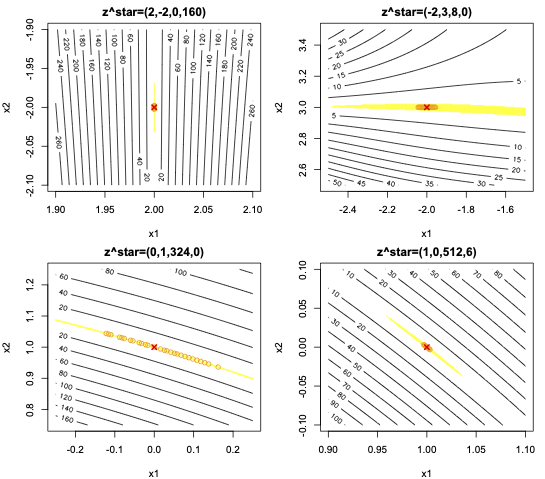
\includegraphics[width=.6\textwidth]{img/4GNEPlots} \label{GNEs} }
\subfloat[The 6 initial points]{ 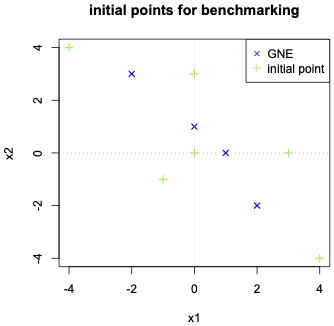
\includegraphics[width=.4\textwidth]{img/4GNEinitialPoints} \label{initpoint} }
\caption{Contour plots of the norm of $\Phi$}
\label{4GNE}
\end{center}
\end{figure}



\subsection{Benchmark of the complementarity functions and the computation methods}
Using the following function, we compare all the different methods with different initial points and different complementarity functions.
We consider the following complementarity functions.
\begin{itemize}
\item $\phi_{Min}(a,b)=\min(a,b)$,
\item $\phi_{FB}(a,b)=\sqrt{a^2+b^2} -(a+b)$,
\item $\phi_{Man}(a,b)=f(|a-b|) - f(a) - f(b)$ and $f(t)=t^3$,
\item $\phi_{LT}(a,b)=(a^q+b^q)^{\frac{1}{q}} -(a+b)$ and $q=4$,
\item $\phi_{KK}(a,b)= (\sqrt{(a-b)^2+2\lambda a b} -(a+b))/(2-\lambda)$ and $\lambda=3/2$.
\end{itemize}
%Firstly, we define a function calling the benchmark function for the five complementarity functions under consideration.
%%%% R code
%<<bench, fig=FALSE, echo=TRUE, eval=FALSE>>=
%wholebench <- function(z0)
%{
%#min function
%resMin <- bench.GNE.nseq(z0, F, JacF, argPhi=list(phi=phiMin), argjac=list(gphia= GrAphiMin, gphib= GrBphiMin), echo=FALSE)
%
%#FB function
%resFB <- bench.GNE.nseq(z0, F, JacF, argPhi=list(phi=phiFB), argjac=list(gphia= GrAphiFB, gphib= GrBphiFB), echo=FALSE)
%
%#Mangasarian function
%resMan <- bench.GNE.nseq(z0, F, JacF, argPhi=list(phi=phiMan, f=function(t) t^3), argjac=list(gphia= GrAphiMan, gphib= GrBphiMan, fprime=function(t) 3*t^2), echo=FALSE, control=list(maxit=200))
%
%#LT function
%resLT <- bench.GNE.nseq(z0, F, JacF, argPhi=list(phi=phiLT, q=4), argjac=list(gphia= GrAphiLT, gphib= GrBphiLT, q=4))
%
%#KK function
%resKK <- bench.GNE.nseq(z0, F, JacF, argPhi=list(phi=phiKK, lambda=3/2), argjac=list(gphia= GrAphiKK, gphib= GrBphiKK, lambda=3/2))
%
%list(resMin=resMin, resFB=resFB, resMan=resMan, resLT=resLT, resKK=resKK)
%}
%@
%%%%
%Then the following call give us a list of result tables.
%%%% R code
%<<benchcall, fig=FALSE, echo=TRUE, eval=FALSE>>=
%initialpt <- cbind(c(4, -4), c(-4, 4), c(3, 0), c(0, 3), c(-1, -1), c(0, 0))
%mytablelist <- list()
%for(i in 1: NCOL(initialpt))
%{
%	z0 <- c(initialpt[, i], 1, 1)
%	mybench <- wholebench(z0)
%
%	cat("z0", z0, "\n")	
%
%	mytable12 <- data.frame(method=mybench[[1]]$compres[, 1], 
%	round( 
%		cbind(mybench[[1]]$compres[,c(-1, -4)], mybench[[2]]$compres[,c(-1, -4)])
%		, 3) )
%
%	mytable35 <- data.frame(method=mybench[[1]]$compres[, 1], 
%	round( 
%		cbind(mybench[[3]]$compres[,c(-1, -4)], mybench[[5]]$compres[,c(-1, -4)])
%		, 3) )
%
%	mytablelist <- c(mytablelist, z0=list(z0), MINFB=list(mytable12), MANKK=list(mytable35))
%}
%@
%%%%
%Note that one result table given by the function \code{bench.GNE.nseq} reports the computation results  for 10 methods given an initial point and a complementarity function. Below an example
%%%% R code
%<<benchessai, fig=FALSE, echo=TRUE, eval=TRUE>>=
%z0 <- c(-4, 4, 1, 1)
%bench.GNE.nseq(z0, F, JacF, argPhi=list(phi=phiMin), argjac=list(gphia= GrAphiMin, gphib= GrBphiMin), echo=FALSE)$compres
%@
%%%%
%The following subsections report the computation for 4 complementarity functions, the Luo-Tseng being discarded due to non convergence. We also remove the final estimates $z_n$ when the method has not converged, $|| \Phi(z_n) ||^2 \neq 0$. Tables are put in appendix, except the first one.


\subsubsection{Initial point $z_0 = (4, -4,  1,  1)$}

We work on the initial point $z_0 = (4, -4,  1,  1)$, close the GNE  $(2, -2, 0, 160)$.
Clearly, we observe the Mangasarian complementarity function $\phi_{Man}$ does not converge except in the pure Newton method, for which the sequence converges to $(-2, 3, 8, 0)$ quite far from the initial point. So the ``Man'' sequence converged by a chance! For $\phi_{Min}$ function, when it converges, the GNEs found are $(2, -2, 0, 160)$ or $(1, 0, 512, 6)$. $\phi_{FB}$ and $\phi_{KK}$ associated sequences converge mostly to  $(2, -2, 0, 160)$. In terms of function/Jacobian calls, $\phi_{FB}$ is significantly better when used with the Newton scheme. 

\begin{table}[htb!]

\begin{scriptsize}
\begin{tabular}{l|ccccccc|ccccccc}
 & \multicolumn{7}{c|}{$\phi_{Min}(a,b)=\min(a,b)$} & \multicolumn{7}{c}{$\phi_{FB}(a,b)=\sqrt{a^2+b^2} -(a+b)$} \\
   &  fctcall  &  jaccall  &  $x_1$  &  $x_2$  &  $\lambda_1$  &  $\lambda_2$  &  $||\Phi(z)||$  &  fctcall  &  jaccall  &  $x_1$  &  $x_2$  &  $\lambda_1$  &  $\lambda_2$  &  $||\Phi(z)||$ \\ 
\hline   
Newton - pure  &   5  &  5  &  1  &  0  &  512  &  6  &  0  &  6  &  6  &  2  &  -2  &  0  &  160  &  0 \\ 
Newton - geom. LS  &   343  &  67  &  1  &  0  &  512  &  6  &  0  &  6  &  6  &  2  &  -2  &  0  &  160  &  0 \\ 
Newton - quad. LS  &   292  &  100  &    &    &    &    &  2  &  6  &  6  &  2  &  -2  &  0  &  160  &  0 \\ 
Newton - Powell TR  &   64  &  57  &  1  &  0  &  512  &  6  &  0  &  12  &  6  &  2  &  -2  &  0  &  160  &  0 \\ 
Newton - Dbl. TR  &   63  &  58  &  1  &  0  &  512  &  6  &  0  &  12  &  6  &  2  &  -2  &  0  &  160  &  0 \\ 
Broyden - pure  &   100  &  1  &    &    &    &    &  164  &  100  &  1  &    &    &    &    &  188 \\ 
Broyden - geom. LS  &   403  &  6  &  1  &  0  &  512  &  6  &  0  &  1079  &  26  &    &    &    &    &  2 \\ 
Broyden - quad. LS  &   291  &  6  &    &    &    &    &  1  &  467  &  3  &    &    &    &    &  1 \\ 
Broyden - Powell TR  &   22  &  2  &  2  &  -2  &  0  &  160  &  0  &  114  &  2  &    &    &    &    &  1 \\ 
Broyden - Dbl. TR  &   20  &  2  &  2  &  -2  &  0  &  160  &  0  &  115  &  2  &    &    &    &    &  1 \\ 
\hline
   &  fctcall  &  jaccall  &  $x_1$  &  $x_2$  &  $\lambda_1$  &  $\lambda_2$  &  $||\Phi(z)||$  &  fctcall  &  jaccall  &  $x_1$  &  $x_2$  &  $\lambda_1$  &  $\lambda_2$  &  $||\Phi(z)||$ \\ 
\hline   
Newton - pure  &   113  &  113  &  -2  &  3  &  8  &  0  &  0  &  48  &  48  &  0  &  1  &  325  &  0  &  0 \\ 
Newton - geom. LS  &   203  &  25  &    &    &    &    &  33  &  727  &  100  &    &    &    &    &  2 \\ 
Newton - quad. LS  &   91  &  27  &    &    &    &    &  37  &  85  &  39  &  2  &  -2  &  0  &  160  &  0 \\ 
Newton - Powell TR  &   75  &  67  &    &    &    &    &  3  &  152  &  100  &  0  &  1  &  309  &  0  &  0 \\ 
Newton - Dbl. TR  &   62  &  53  &    &    &    &    &  3  &  147  &  100  &  0  &  1  &  304  &  0  &  0 \\ 
Broyden - pure  &   200  &  1  &    &    &    &    &  506  &  49  &  1  &  1  &  0  &  512  &  6  &  0 \\ 
Broyden - geom. LS  &   167  &  6  &    &    &    &    &  82  &  29  &  3  &  2  &  -2  &  0  &  160  &  0 \\ 
Broyden - quad. LS  &   86  &  5  &    &    &    &    &  78  &  20  &  3  &  2  &  -2  &  0  &  160  &  0 \\ 
Broyden - Powell TR  &   215  &  14  &    &    &    &    &  3  &  28  &  2  &  2  &  -2  &  0  &  160  &  0 \\ 
Broyden - Dbl. TR  &   246  &  15  &    &    &    &    &  3  &  29  &  2  &  2  &  -2  &  0  &  160  &  0 \\ 
\hline
& \multicolumn{7}{c|}{$\phi_{Man}(a,b)=f(|a-b|) - f(a) - f(b)$ and $f(t)=t^3$} & 
\multicolumn{7}{c}{$\phi_{KK}(a,b)= (\sqrt{(a-b)^2+2\lambda a b} -(a+b))/(2-\lambda)$ and $\lambda=3/2$} \\
\end{tabular}
\end{scriptsize}

\caption{With initial point $z_0 = (4, -4,  1,  1)$ close to $(2, -2, 0, 160)$}
\label{bench4m411}

\end{table}


\subsubsection{Initial point $z_0 = (-4, 4,  1,  1)$}

We work on the initial point $z_0 = (-4, 4,  1,  1)$, close the GNE  $(-2, 3, 8, 0)$.
Again, we observe the Mangasarian complementarity function $\phi_{Man}$ does not converge. All other sequences converge the closest GNE $(-2, 3, 8, 0)$. $\phi_{Min}$ sequence with Newton scheme is particularly good, then comes $\phi_{FB}$ and finally $\phi_{KK}$.





\subsubsection{Initial point $z_0 = (3, 0,  1,  1)$}

We work on the initial point $z_0 = (3, 0,  1,  1)$ close to the GNE $(1, 0, 512, 6)$. As always, the ``Man'' sequence converges by chance with the pure Newton method to a GNE $(-2, 3, 8, 0)$. Otherwise the other sequences, namely ``Min'', ``FB'' and ``KK'' converges to the expected GNE. As the previous subsection, Broyden updates of the Jacobian is less performant than the true Jacobian (i.e. Newton scheme). The convergence speed order is preserved.






\subsubsection{Initial point $z_0 = (0, 3, 1, 1)$}

We work on the initial point $z_0 = (0, 3, 1,  1)$ close to the GNE $(0, 1, 324, 0)$. As always, the ``Man'' sequence converges by chance with the pure Newton method to a GNE $(-2, 3, 8, 0)$. Others sequences have difficulty to converge the closest GNE. Local methods (i.e. pure) find the GNE $(0, 1, 324, 0)$, while global version converges to $(1, 0, 512, 6)$. It is logical any method will have difficulty to choose between these two GNEs, because they are close. 



\subsubsection{Initial point $z_0 = (-1, -1, 1,  1)$}

We work on the initial point $z_0 = (-1, -1, 1,  1)$ equidistant to the GNEs $(0, 1, 324, 0)$ and $(1, 0, 512, 6)$. Despite being closer to these GNEs, the pure Newton version of the ``Man'' sequence converges unconditionally to the GNE $(-2, 3, 8, 0)$. All other sequences converges to the GNE $(0, 1, 324, 0)$  except for the Broyden version of the ``KK'' sequence, converging to the farthest GNEs. In terms of function calls, the Newton line search version of the ``Min'' sequence is the best, followed by the Newton trust region version of the ``FB'' sequence.



\subsubsection{Initial point $z_0 = (0, 0, 1,  1)$}

We work on the initial point $z_0 = (0, 0, 1,  1)$ equidistant to the GNEs $(0, 1, 324, 0)$ and $(1, 0, 512, 6)$. Both the ``Man'' and the ``Min'' sequences do not converge. The ``Min'' sequence diverges because the Jacobian at the initial point is exactly singular. Indeed, we have
%%% R code
\begin{Schunk}
\begin{Sinput}
> z0 <- c(0, 0, 1, 1)
> jacSSR(z0, dimx, dimlam, heobj=heobj, myarg, constr=g, grconstr=grg, 
+ 	heconstr=heg, gcompla=GrAphiMin, gcomplb=GrBphiMin)
\end{Sinput}
\begin{Soutput}
     [,1] [,2] [,3] [,4]
[1,]  512 1024    1    0
[2,]    0    0    0    2
[3,]   -1   -1    1    0
[4,]    0    0    0    1
\end{Soutput}
\end{Schunk}
%%%
For the ``FB'' and ``KK'' sequences, we do not have this problem.
%%% R code
\begin{Schunk}
\begin{Sinput}
> jacSSR(z0, dimx, dimlam, heobj=heobj, myarg, constr=g, grconstr=grg, 
+ 	heconstr=heg, gcompla=GrAphiFB, gcomplb=GrBphiFB)
\end{Sinput}
\begin{Soutput}
            [,1]         [,2]       [,3]       [,4]
[1,] 512.0000000 1024.0000000  1.0000000  0.0000000
[2,]   0.0000000    0.0000000  0.0000000  2.0000000
[3,]   0.2928932    0.2928932 -0.2928932  0.0000000
[4,]   0.1055728    0.2111456  0.0000000 -0.5527864
\end{Soutput}
\begin{Sinput}
> jacSSR(z0, dimx, dimlam, heobj=heobj, myarg, constr=g, grconstr=grg, 
+ 	heconstr=heg, gcompla=GrAphiKK, gcomplb=GrBphiKK, argcompl=3/2)
\end{Sinput}
\begin{Soutput}
            [,1]         [,2]       [,3]       [,4]
[1,] 512.0000000 1024.0000000  1.0000000  0.0000000
[2,]   0.0000000    0.0000000  0.0000000  2.0000000
[3,]   0.2679492    0.2679492 -0.2679492  0.0000000
[4,]   0.1101776    0.2203553  0.0000000 -0.4881421
\end{Soutput}
\end{Schunk}
%%%
So the sequence converge to a GNE, either $(0, 1, 324, 0)$ or $(-2, 3, 8, 0)$. Again the ``KK'' sequence converges faster.


\subsubsection{Conclusions}
In conclusion to this analysis with respect to initial point, the computation method and the complementarity function, we observe the strong difference in terms of convergence, firstly and in terms of convergence speed. Clearly the choice of the complementarity function is crucial, the Luo-Tseng and the Mangasarian are particularly inadequate in our example. Regarding the remaining three complementarity functions (the minimum, the Fisher-Burmeister and the Kanzow-Kleinmichel functions) generally converge irrespectively of the computation method. However, the ``KK'' sequences are particularly efficient and most of the time the Newton trust region method is the best in terms of function/Jacobian calls.



\subsection{Special case of shared constraints with common multipliers}

Let $h:  \R^{n} \mapsto  \R^{m_l}$ be a constraint function shared by all players. 
The total constraint function and the Lagrange multiplier for the $i$th player is 
$$
\tilde g^i(x) = 
\left( \begin{matrix}
g^i(x) \\
h(x) 
\end{matrix} \right)
\txtm{and}
\tilde \lambda^i = 
\left( \begin{matrix}
\lambda^i \\
\mu
\end{matrix} \right),
$$
where $\mu \in \R^l$.
This could fall within the previous framework, if we have not required the bottom part of $\tilde \lambda^i$ to be common among all players. 
The Lagrangian function of the $i$th player is given by
$$
L ^i(x, \lambda^i, \mu) = O_i(x) + \sum_{k=1}^{m_i} g^i_k(x) \lambda_k^i + \sum_{p=1}^l h_p(x) \mu_p.
$$

\begin{mydef}[eKKTc]
For the $N$ optimization subproblems for the functions $\theta_i: \R^{n} \mapsto \R$, with constraints $g_i: \R^{n} \mapsto \R^{m_i}$ and shared constraint $h:\R^n \mapsto \R^l$, the KKT conditions can be regrouped such that
there exists $\lambda \in \R^m$ and 
$$
\bar L(x, \lambda, \mu) = 0 \txtm{and} 0 \leq \lambda, 0 \leq \mu \perp g(x) \leq  0,
$$
where $L$ and $G$ are given by
$$
\bar L(x, \lambda, \mu) = 
\left( 
\begin{matrix}
\nabla_{x_1} L ^1(x, \lambda^1, \mu) \\
\vdots \\
\nabla_{x_I} L ^I(x, \lambda^I, \mu) \\
\end{matrix}
\right)  
\in \R^{n}
\txtm{and}
g(x) = 
\left( 
\begin{matrix}
g^1(x) \\
\vdots \\
g^N(x) \\
h(x) 
\end{matrix}
\right) 
\in \R^{m}.
$$
The extended KKT system is denoted by eKKTc($N, \theta_i, g_i, h$).
\end{mydef}
The generalized Jacobian is given in Appendix \ref{app:nseq:jointcase}.




\subsection{Constrained-equation reformulation of the KKT system}
This subsection aims to present methods specific to solve constrained (nonlinear) equations, first proposed by \cite{kanzowfacchetal11} in the GNEP context.
The root function $H: \R^n \times \R^{2m} \mapsto  \R^n \times \R^{2m}$ is defined as
$$
H(x, \lambda, w) = 
\left( 
\begin{matrix}
\tilde L(x, \lambda) \\
g(x) + w \\
\lambda \circ w 
\end{matrix}
\right) ,
$$
where the dimensions $n, m$ correspond to the GNEP notation ($ \lambda = (\lambda^1, \dots, \lambda^N)$) and $(a, \bar \sigma)$ is given by $((0_{n}, \II_{m}), 1)$. The potential function is given by
$$
p\left(u \right) = \zeta \log\left( ||x||_2^2 + ||\lambda ||_2^2+ ||w||_2^2 \right) - 
\sum_{k=1}^{m} \log (\lambda_{k}) - \sum_{k=1}^{m} \log (w_{k}),
$$
where $u=(x, \lambda, w) \in \R^n \times \R_{+}^{m} \times \R_{+}^{m}$
and $\zeta > m$. 
The Jacobian is given in Appendix \ref{app:ceq:gencase}.

When there is a constraint function $h$ shared by all players, the root function is given by
$$
\widetilde H(x, \tilde \lambda, \tilde w) = 
\left( 
\begin{matrix}
\bar L(x, \tilde \lambda) \\
\tilde g(x) + \tilde w \\
\tilde \lambda \circ \tilde w 
\end{matrix}
\right) ,
\txtm{with}
\tilde \lambda = 
\left( 
\begin{matrix}
\lambda^1 \\
\vdots \\
\lambda^N \\
\mu
\end{matrix}
\right) 
,
\tilde w = 
\left( 
\begin{matrix}
w^1 \\
\vdots \\
w^N \\
y
\end{matrix}
\right) 
\txtm{and}
\tilde g(x) = 
\left( 
\begin{matrix}
g^1(x) \\
\vdots \\
g^N(x) \\
h(x)
\end{matrix}
\right) .
$$
The Jacobian is given in Appendix \ref{app:ceq:jointcase}.





\subsubsection{A classic example}
Using the classic example presented above, we get

Therefore, to compute a generalized Nash equilibrium, we use
%%% R code
\begin{Schunk}
\begin{Sinput}
> z0 <- 1+rexp(sum(dimx)+2*sum(dimlam))
> GNE.ceq(z0, dimx, dimlam, grobj=grobj, myarg, heobj=heobj, myarg, 
+ 	constr=g, grconstr=grg, heconstr=heg, 
+ 	method="PR", control=list(trace=0))
\end{Sinput}
\begin{Soutput}
GNE: 4.109111 1.41207 3.350895 28.05423 1.326807 0.1310603 
with optimal norm 870.9463 
after  55 iterations with exit code 3 .
Output message: No better point found (algorithm has stalled) 
Function/grad/hessian calls: 720 55 
Optimal (vector) value: 192.559 -849.3178 5.847988 7.761353 4.44599 3.676795 
\end{Soutput}
\end{Schunk}
%%%




%________________________________________________________________________
\section{GNEP as a fixed point equation}
%________________________________________________________________________

We present a last reformulation of the GNEP, which was originally introduced in the context of standard Nash equilibrium problem. 
We define the Nikaido-Isoda function as the function $\psi$ from $\R^{2n}$ to  $\R$ by
\begin{equation}
\psi(x, y) = \sum_{\nu = 1}^N [ \theta(x_\nu, x_{-\nu}) -  \theta(y_\nu, x_{-\nu}) ].
\label{eq:NIF}
\end{equation}
This function represents the unilateral player  improvement of the objective function between actions $x$ and $y$. 
Let $\hat V$ be the gap function 
$$
\hat V(x) = \underset{ y \in X(x) }{\sup}~ \psi(x,y).
$$
Theorem 3.2 of \cite{facchkanz09b} shows the relation between GNEPs and the Nikaido-Isoda function. 
If objective functions $\theta_i$ are continuous, then  $x^\star$ solves the GNEP if and only if $x^\star$ solves the equation 
\begin{equation}
\hat V(x) = 0
\txtm{and} 
x \in X(x),
\label{eq:NIF:general}
\end{equation}
where the set $X(x) = \{y \in \R^n, \forall i, g^i(y_i, x_{-i}) \leq 0 \}$ and $\hat V$ defined in (\ref{eq:NIF}). Furthermore, the function $\hat V$ is such that $\forall x \in X(x), \hat V(x) \geq 0$.
There is no particular algorithm able to solve this problem for a general constrained set $X(x)$. But a simplification will occur in a special case.



\subsection{The jointly convex case}

In this subsection, we present reformulations for a subclass of GNEP called jointly convex case. 
Firstly, the jointly convex setting requires that the constraint function is common to all players $g^1=\dots =g^N= g$.
Then, we assume, there exists a closed convex subset $X \subset \R^n$ such that for all player $i$, 
$$
\{y_i \in \R^{n_i},  g(y_i, x_{-i}) \leq 0 \} 
=
\{y_i \in \R^{n_i},  (y_i, x_{-i}) \in X \} .  
$$ 
The convexity of $X$ implies that the constraint function $g$ is  quasiconvex with respect to all variables.
However, we generally assume that $g$ is convex with respect to all variables.


%**************
\subsubsection{NIF formulation for the jointly convex case}



Recalling that for the Nikaido-Isoda function (\ref{eq:NIF}), the gap function is
$$
\hat V(x) = \underset{ y \in X(x) }{\sup}~ \psi(x,y).
$$
In the jointly convex case, we get
\begin{equation}
\hat V(x) = 0
\txtm{and} 
x \in X(x),
\label{eq:NIF:joint}
\end{equation}
where the set $X(x) = \{y \in \R^n, g(y_i, x_{-i}) \leq 0 \}$. Still the computation of $\hat V$ is a complex optimization over a constrained set $X(x)$.
As in the previous subsection, the class of GNE called variational equilibrium can be characterized by the NI formulation.  We have the folllowing theorem.


Assuming $\theta_i$ and $g$ are C\expo{1} functions and $g$ is convex and $\theta_i$ player-convex. $x^\star$ is a variational equilibrium if and only if $x^\star \in X$ and $V(x^\star)=0$ with $V$ defined as
$$
V(x) = \underset{ y \in X }{\sup}~ \psi(x,y).
$$








%________________________________________________________________________
\section{GNEP as a gap minimization problem}
%________________________________________________________________________






%________________________________________________________________________
\section{List of examples}
%________________________________________________________________________

\subsection{Example of \cite{facchineietal07}}
We consider a two-player game defined by 
$$
O_1(x) = (x_1-1)^2 
\txtm{and}
O_2(x) = (x_2-1/2)^2,  
$$
with a shared constraint function
$$
g(x) = x_1 + x_2 - 1 \leq 0.
$$
Solutions are given by $(\alpha, 1-\alpha)$ with $\alpha \in [1/2, 1]$ with Lagrange multipliers given by $\lambda_1 = 2 - 2\alpha$ and $\lambda_2 = 2\alpha - 1$.
But there is a unique normalized equilibrium for which $\lambda_1=\lambda_2=1/2$.
The nonsmooth reformulation of the KKT system uses the following terms
$$
\nabla_1 O_1(x) = 2(x_1-1),
\nabla_2 O_2(x) = 2(x_2-1/2),
\txtm{and}
\nabla_1 g(x) = \nabla_2 g(x) = 1.
$$
and 
$$
\nabla_i^2 O_i(x) = 2,
\nabla_j \nabla_k O_i(x) = 0,
\txtm{and}
\nabla_j \nabla_k g(x) = 0.
$$

\subsection{The Duopoly game from \cite{krawuryasev00}}
We consider a two-player game defined by 
$$
O_i(x) = - (d- \lambda -\rho(x_1+x_2))x_i,
$$
with 
$$
g_i(x) = -x_i \leq 0,
$$
where $d = 20$, $\lambda = 4$, $\rho = 1$.
Derivatives are given by
$$
\nabla_j O_i(x) = -( -\rho x_i + (d- \lambda -\rho(x_1+x_2))\delta_{ij} )
\txtm{and}
\nabla_j g_i(x) = - \delta_{ij},
$$
and
$$
\nabla_k \nabla_j O_i(x) = -( -\rho \delta_{ik} - \rho\delta_{ij})
\txtm{and}
\nabla_k \nabla_j g_i(x) = 0.
$$
There is a unique solution given by $x^\star = (d-\lambda)/(3\rho)$.

\subsection{The River basin pollution game from \cite{krawuryasev00}}
We consider a two-player game defined by 
$$
O_i(x) = - (d_1 - d_2 (x_1+x_2+x_3) - c_{1i} - c_{2i} x_i)x_i,
$$
and
$$
g(x) = 
\left( \begin{matrix}
\sum\limits_{l=1}^3 u_{l1} e_l x_l - K_1 \\
\sum\limits_{l=1}^3 u_{l2} e_l x_l - K_2 
\end{matrix} \right).
$$
Derivatives are given by
$$
\nabla_j O_i(x) = - ( - d_2  - c_{2i} \delta_{ij})x_i - (d_1 - d_2 (x_1+x_2+x_3) - c_{1i} - c_{2i} x_i)\delta_{ij}
\txtm{and}
\nabla_j g(x) = 
\left( \begin{matrix}
u_{j1} e_j  \\
u_{j2} e_j
\end{matrix} \right),
$$
and
$$
\nabla_k \nabla_j O_i(x) = -( - d_2\delta_{ik} - d_2\delta_{ij}  - 2 c_{2i} \delta_{ij}\delta_{ik})
\txtm{and}
\nabla_k \nabla_j g(x) = 
\left( \begin{matrix}
0 & 0  \\
0 & 0
\end{matrix} \right).
$$




\newpage
\bibliographystyle{agsm}
\bibliography{GNE-howto}


%________________________________________________________________________%________________________________________________________________________
\appendix


%%________________________________________________________________________
%\section{Tables for the nonsmooth reformulation}
%%________________________________________________________________________
%
%
%\begin{table}[htb!]
%
%\begin{scriptsize}
%\begin{tabular}{l|ccccccc|ccccccc}
% & \multicolumn{7}{c|}{$\phi_{Min}(a,b)=\min(a,b)$} & \multicolumn{7}{c}{$\phi_{FB}(a,b)=\sqrt{a^2+b^2} -(a+b)$} \\
%   &  fctcall  &  jaccall  &  $x_1$  &  $x_2$  &  $\lambda_1$  &  $\lambda_2$  &  $||\Phi(z)||$  &  fctcall  &  jaccall  &  $x_1$  &  $x_2$  &  $\lambda_1$  &  $\lambda_2$  &  $||\Phi(z)||$ \\ 
%\hline   
%Newton - pure  &   7  &  7  &  -2  &  3  &  8  &  0  &  0  &  9  &  9  &  -2  &  3  &  8  &  0  &  0 \\ 
%Newton - geom. LS  &   7  &  7  &  -2  &  3  &  8  &  0  &  0  &  10  &  9  &  -2  &  3  &  8  &  0  &  0 \\ 
%Newton - quad. LS  &   7  &  7  &  -2  &  3  &  8  &  0  &  0  &  11  &  10  &  -2  &  3  &  8  &  0  &  0 \\ 
%Newton - Powell TR  &   8  &  7  &  -2  &  3  &  8  &  0  &  0  &  13  &  10  &  -2  &  3  &  8  &  0  &  0 \\ 
%Newton - Dbl. TR  &   8  &  7  &  -2  &  3  &  8  &  0  &  0  &  13  &  10  &  -2  &  3  &  8  &  0  &  0 \\ 
%Broyden - pure  &   35  &  1  &  -2  &  3  &  8  &  0  &  0  &  35  &  1  &  -2  &  3  &  8  &  0  &  0 \\ 
%Broyden - geom. LS  &   30  &  3  &  -2  &  3  &  8  &  0  &  0  &  39  &  4  &  -2  &  3  &  8  &  0  &  0 \\ 
%Broyden - quad. LS  &   26  &  3  &  -2  &  3  &  8  &  0  &  0  &  30  &  4  &  -2  &  3  &  8  &  0  &  0 \\ 
%Broyden - Powell TR  &   169  &  6  &    &    &    &    &  1  &  26  &  2  &  -2  &  3  &  8  &  0  &  0 \\ 
%Broyden - Dbl. TR  &   182  &  6  &    &    &    &    &  1  &  28  &  2  &  -2  &  3  &  8  &  0  &  0 \\ 
%
%\hline
%   &  fctcall  &  jaccall  &  $x_1$  &  $x_2$  &  $\lambda_1$  &  $\lambda_2$  &  $||\Phi(z)||$  &  fctcall  &  jaccall  &  $x_1$  &  $x_2$  &  $\lambda_1$  &  $\lambda_2$  &  $||\Phi(z)||$ \\ 
%\hline   
%Newton - pure  &   200  &  200  &    &    &    &    &  53  &  11  &  11  &  -2  &  3  &  8  &  0  &  0 \\ 
%Newton - geom. LS  &   66  &  10  &    &    &    &    &  4  &  11  &  10  &  -2  &  3  &  8  &  0  &  0 \\ 
%Newton - quad. LS  &   25  &  9  &    &    &    &    &  3  &  19  &  14  &  -2  &  3  &  8  &  0  &  0 \\ 
%Newton - Powell TR  &   47  &  40  &    &    &    &    &  3  &  10  &  10  &  -2  &  3  &  8  &  0  &  0 \\ 
%Newton - Dbl. TR  &   44  &  36  &    &    &    &    &  3  &  10  &  10  &  -2  &  3  &  8  &  0  &  0 \\ 
%Broyden - pure  &   200  &  1  &    &    &    &    &  73  &  39  &  1  &  -2  &  3  &  8  &  0  &  0 \\ 
%Broyden - geom. LS  &   1045  &  25  &    &    &    &    &  3  &  75  &  3  &  -2  &  3  &  8  &  0  &  0 \\ 
%Broyden - quad. LS  &   253  &  11  &    &    &    &    &  4  &  42  &  3  &  -2  &  3  &  8  &  0  &  0 \\ 
%Broyden - Powell TR  &   156  &  12  &    &    &    &    &  3  &  33  &  3  &  -2  &  3  &  8  &  0  &  0 \\ 
%Broyden - Dbl. TR  &   108  &  8  &    &    &    &    &  3  &  36  &  2  &  -2  &  3  &  8  &  0  &  0 \\ 
%\hline
%& \multicolumn{7}{c|}{$\phi_{Man}(a,b)=f(|a-b|) - f(a) - f(b)$ and $f(t)=t^3$} & 
%\multicolumn{7}{c}{$\phi_{KK}(a,b)= (\sqrt{(a-b)^2+2\lambda a b} -(a+b))/(2-\lambda)$ and $\lambda=3/2$} \\
%
%\end{tabular}
%\end{scriptsize}
%
%\caption{With initial point $z_0 = (-4, 4,  1,  1)$ close to $(-2, 3, 8, 0)$}
%\label{benchm4411}
%
%\end{table}
%
%
%
%
%\begin{table}[htb!]
%
%\begin{scriptsize}
%\begin{tabular}{l|ccccccc|ccccccc}
% & \multicolumn{7}{c|}{$\phi_{Min}(a,b)=\min(a,b)$} & \multicolumn{7}{c}{$\phi_{FB}(a,b)=\sqrt{a^2+b^2} -(a+b)$} \\
%   &  fctcall  &  jaccall  &  $x_1$  &  $x_2$  &  $\lambda_1$  &  $\lambda_2$  &  $||\Phi(z)||$  &  fctcall  &  jaccall  &  $x_1$  &  $x_2$  &  $\lambda_1$  &  $\lambda_2$  &  $||\Phi(z)||$ \\ 
%\hline   
%Newton - pure  &   22  &  22  &  0  &  1  &  325  &  0  &  0  &  21  &  21  &  2  &  -2  &  0  &  160  &  0 \\ 
%Newton - geom. LS  &   25  &  24  &  0  &  1  &  325  &  0  &  0  &  25  &  24  &  0  &  1  &  325  &  0  &  0 \\ 
%Newton - quad. LS  &   13  &  9  &  2  &  -2  &  0  &  160  &  0  &  197  &  100  &  0  &  1  &  345  &  0  &  0 \\ 
%Newton - Powell TR  &   26  &  24  &  0  &  1  &  325  &  0  &  0  &  12  &  8  &  1  &  0  &  512  &  6  &  0 \\ 
%Newton - Dbl. TR  &   26  &  24  &  0  &  1  &  325  &  0  &  0  &  13  &  9  &  1  &  0  &  512  &  6  &  0 \\ 
%Broyden - pure  &   6  &  1  &    &    &    &    &  2e+25  &  100  &  1  &    &    &    &    &  4 \\ 
%Broyden - geom. LS  &   58  &  3  &  1  &  0  &  512  &  6  &  0  &  639  &  4  &    &    &    &    &  12 \\ 
%Broyden - quad. LS  &   389  &  3  &  1  &  0  &  512  &  6  &  0  &  187  &  3  &  1  &  0  &  512  &  6  &  0 \\ 
%Broyden - Powell TR  &   164  &  2  &  0  &  1  &  376  &  0  &  0  &  133  &  2  &    &    &    &    &  1 \\ 
%Broyden - Dbl. TR  &   144  &  3  &  0  &  1  &  343  &  0  &  0  &  138  &  2  &    &    &    &    &  1 \\ 
%\hline
%
%   &  fctcall  &  jaccall  &  $x_1$  &  $x_2$  &  $\lambda_1$  &  $\lambda_2$  &  $||\Phi(z)||$  &  fctcall  &  jaccall  &  $x_1$  &  $x_2$  &  $\lambda_1$  &  $\lambda_2$  &  $||\Phi(z)||$ \\ 
%\hline   
%Newton - pure  &   76  &  76  &  -2  &  3  &  8  &  0  &  0  &  66  &  66  &  -2  &  3  &  8  &  0  &  0 \\ 
%Newton - geom. LS  &   176  &  17  &    &    &    &    &  50  &  45  &  17  &  2  &  -2  &  0  &  160  &  0 \\ 
%Newton - quad. LS  &   1121  &  200  &    &    &    &    &  113  &  130  &  45  &  2  &  -2  &  0  &  160  &  0 \\ 
%Newton - Powell TR  &   72  &  61  &    &    &    &    &  3  &  38  &  25  &  2  &  -2  &  0  &  160  &  0 \\ 
%Newton - Dbl. TR  &   64  &  55  &    &    &    &    &  3  &  41  &  26  &  2  &  -2  &  0  &  160  &  0 \\ 
%Broyden - pure  &   200  &  1  &    &    &    &    &  5.9e6  &  85  &  1  &    &    &    &    &  393 \\ 
%Broyden - geom. LS  &   349  &  9  &    &    &    &    &  64  &  806  &  3  &    &    &    &    &  3 \\ 
%Broyden - quad. LS  &   123  &  9  &    &    &    &    &  58  &  202  &  3  &  1  &  0  &  512  &  6  &  0 \\ 
%Broyden - Powell TR  &   101  &  6  &  -2  &  3  &  8  &  0  &  0  &  121  &  4  &  1  &  0  &  512  &  6  &  0 \\ 
%Broyden - Dbl. TR  &   180  &  14  &    &    &    &    &  3  &  157  &  6  &  2  &  -2  &  0  &  160  &  0 \\ 
%\hline
%& \multicolumn{7}{c|}{$\phi_{Man}(a,b)=f(|a-b|) - f(a) - f(b)$ and $f(t)=t^3$} & 
%\multicolumn{7}{c}{$\phi_{KK}(a,b)= (\sqrt{(a-b)^2+2\lambda a b} -(a+b))/(2-\lambda)$ and $\lambda=3/2$} \\
%
%\end{tabular}
%\end{scriptsize}
%
%\caption{With initial point $z_0 = (3, 0,  1,  1)$ close to $(1, 0, 512, 6)$}
%\label{bench3011}
%
%\end{table}
%
%
%\begin{table}[htb!]
%
%\begin{scriptsize}
%\begin{tabular}{l|ccccccc|ccccccc}
% & \multicolumn{7}{c|}{$\phi_{Min}(a,b)=\min(a,b)$} & \multicolumn{7}{c}{$\phi_{FB}(a,b)=\sqrt{a^2+b^2} -(a+b)$} \\
%   &  fctcall  &  jaccall  &  $x_1$  &  $x_2$  &  $\lambda_1$  &  $\lambda_2$  &  $||\Phi(z)||$  &  fctcall  &  jaccall  &  $x_1$  &  $x_2$  &  $\lambda_1$  &  $\lambda_2$  &  $||\Phi(z)||$ \\ 
%\hline   
%Newton - pure  &   22  &  22  &  0  &  1  &  325  &  0  &  0  &  5  &  5  &  1  &  0  &  512  &  6  &  0 \\ 
%Newton - geom. LS  &   522  &  82  &  1  &  0  &  512  &  6  &  0  &  779  &  100  &    &    &    &    &  1 \\ 
%Newton - quad. LS  &   300  &  100  &    &    &    &    &  2  &  366  &  100  &    &    &    &    &  1 \\ 
%Newton - Powell TR  &   88  &  67  &  1  &  0  &  512  &  6  &  0  &  94  &  73  &  1  &  0  &  512  &  6  &  0 \\ 
%Newton - Dbl. TR  &   102  &  80  &  1  &  0  &  512  &  6  &  0  &  87  &  80  &  0  &  1  &  323  &  0  &  0 \\ 
%Broyden - pure  &   8  &  1  &    &    &    &    &  2e+20  &  100  &  1  &    &    &    &    &  617 \\ 
%Broyden - geom. LS  &   746  &  3  &    &    &    &    &  3  &  844  &  3  &    &    &    &    &  1 \\ 
%Broyden - quad. LS  &   312  &  3  &    &    &    &    &  3  &  345  &  3  &    &    &    &    &  1 \\ 
%Broyden - Powell TR  &   169  &  4  &    &    &    &    &  1  &  40  &  2  &  -2  &  3  &  8  &  0  &  0 \\ 
%Broyden - Dbl. TR  &   158  &  1  &    &    &    &    &  2  &  35  &  2  &  -2  &  3  &  8  &  0  &  0 \\ 
%\hline
%
%   &  fctcall  &  jaccall  &  $x_1$  &  $x_2$  &  $\lambda_1$  &  $\lambda_2$  &  $||\Phi(z)||$  &  fctcall  &  jaccall  &  $x_1$  &  $x_2$  &  $\lambda_1$  &  $\lambda_2$  &  $||\Phi(z)||$ \\ 
%\hline   
%Newton - pure  &   136  &  136  &  -2  &  3  &  8  &  0  &  0  &  24  &  24  &  0  &  1  &  325  &  0  &  0 \\ 
%Newton - geom. LS  &   156  &  14  &    &    &    &    &  14  &  762  &  100  &    &    &    &    &  2 \\ 
%Newton - quad. LS  &   33  &  8  &    &    &    &    &  14  &  358  &  100  &    &    &    &    &  1 \\ 
%Newton - Powell TR  &   31  &  25  &    &    &    &    &  3  &  90  &  72  &  1  &  0  &  512  &  6  &  0 \\ 
%Newton - Dbl. TR  &   35  &  29  &    &    &    &    &  3  &  89  &  76  &  1  &  0  &  512  &  6  &  0 \\ 
%Broyden - pure  &   30  &  1  &    &    &    &    &  9e+33  &  18  &  1  &    &    &    &    &  4e+21 \\ 
%Broyden - geom. LS  &   327  &  10  &    &    &    &    &  13  &  659  &  4  &    &    &    &    &  1 \\ 
%Broyden - quad. LS  &   139  &  10  &    &    &    &    &  13  &  326  &  3  &    &    &    &    &  1 \\ 
%Broyden - Powell TR  &   175  &  14  &    &    &    &    &  3  &  35  &  2  &  -2  &  3  &  8  &  0  &  0 \\ 
%Broyden - Dbl. TR  &   130  &  11  &    &    &    &    &  3  &  53  &  2  &  -2  &  3  &  8  &  0  &  0 \\ 
%\hline
%& \multicolumn{7}{c|}{$\phi_{Man}(a,b)=f(|a-b|) - f(a) - f(b)$ and $f(t)=t^3$} & 
%\multicolumn{7}{c}{$\phi_{KK}(a,b)= (\sqrt{(a-b)^2+2\lambda a b} -(a+b))/(2-\lambda)$ and $\lambda=3/2$} \\
%
%\end{tabular}
%\end{scriptsize}
%
%\caption{With initial point $z_0 = (0, 3, 1,  1)$ close to $(0, 1, 324, 0)$}
%\label{bench0311}
%
%\end{table}
%
%
%
%\begin{table}[htb!]
%
%\begin{scriptsize}
%\begin{tabular}{l|ccccccc|ccccccc}
% & \multicolumn{7}{c|}{$\phi_{Min}(a,b)=\min(a,b)$} & \multicolumn{7}{c}{$\phi_{FB}(a,b)=\sqrt{a^2+b^2} -(a+b)$} \\
%   &  fctcall  &  jaccall  &  $x_1$  &  $x_2$  &  $\lambda_1$  &  $\lambda_2$  &  $||\Phi(z)||$  &  fctcall  &  jaccall  &  $x_1$  &  $x_2$  &  $\lambda_1$  &  $\lambda_2$  &  $||\Phi(z)||$ \\ 
%\hline   
%Newton - pure  &   21  &  21  &  0  &  1  &  323  &  0  &  0  &  9  &  9  &  0  &  1  &  324  &  0  &  0 \\ 
%Newton - geom. LS  &   21  &  21  &  0  &  1  &  323  &  0  &  0  &  194  &  52  &  0  &  1  &  323  &  0  &  0 \\ 
%Newton - quad. LS  &   21  &  21  &  0  &  1  &  323  &  0  &  0  &  154  &  68  &  0  &  1  &  323  &  0  &  0 \\ 
%Newton - Powell TR  &   84  &  70  &  0  &  1  &  323  &  0  &  0  &  32  &  30  &  0  &  1  &  323  &  0  &  0 \\ 
%Newton - Dbl. TR  &   78  &  70  &  0  &  1  &  323  &  0  &  0  &  32  &  30  &  0  &  1  &  323  &  0  &  0 \\ 
%Broyden - pure  &   100  &  1  &  0  &  1  &  307  &  0  &  0  &  37  &  1  &    &    &    &    &  408 \\ 
%Broyden - geom. LS  &   49  &  3  &  0  &  1  &  323  &  0  &  0  &  407  &  6  &  1  &  0  &  512  &  6  &  0 \\ 
%Broyden - quad. LS  &   56  &  4  &  0  &  1  &  302  &  0  &  0  &  324  &  6  &    &    &    &    &  1 \\ 
%Broyden - Powell TR  &   169  &  5  &    &    &    &    &  1  &  183  &  4  &    &    &    &    &  1 \\ 
%Broyden - Dbl. TR  &   172  &  5  &    &    &    &    &  1  &  191  &  4  &    &    &    &    &  1 \\ 
%\hline
%
%   &  fctcall  &  jaccall  &  $x_1$  &  $x_2$  &  $\lambda_1$  &  $\lambda_2$  &  $||\Phi(z)||$  &  fctcall  &  jaccall  &  $x_1$  &  $x_2$  &  $\lambda_1$  &  $\lambda_2$  &  $||\Phi(z)||$ \\ 
%\hline   
%Newton - pure  &   59  &  59  &  -2  &  3  &  8  &  0  &  0  &  18  &  18  &  0  &  1  &  323  &  0  &  0 \\ 
%Newton - geom. LS  &   67  &  11  &    &    &    &    &  5  &  170  &  48  &  0  &  1  &  323  &  0  &  0 \\ 
%Newton - quad. LS  &   42  &  14  &    &    &    &    &  5  &  132  &  60  &  0  &  1  &  323  &  0  &  0 \\ 
%Newton - Powell TR  &   55  &  49  &    &    &    &    &  3  &  87  &  72  &  1  &  0  &  512  &  6  &  0 \\ 
%Newton - Dbl. TR  &   46  &  40  &    &    &    &    &  3  &  87  &  79  &  0  &  1  &  323  &  0  &  0 \\ 
%Broyden - pure  &   200  &  1  &    &    &    &    &  6  &  100  &  1  &    &    &    &    &  168 \\ 
%Broyden - geom. LS  &   836  &  14  &    &    &    &    &  5  &  50  &  4  &  -2  &  3  &  8  &  0  &  0 \\ 
%Broyden - quad. LS  &   89  &  9  &    &    &    &    &  3  &  43  &  3  &  -2  &  3  &  8  &  0  &  0 \\ 
%Broyden - Powell TR  &   113  &  10  &    &    &    &    &  3  &  146  &  6  &  2  &  -2  &  0  &  160  &  0 \\ 
%Broyden - Dbl. TR  &   98  &  7  &    &    &    &    &  3  &  136  &  7  &  2  &  -2  &  0  &  160  &  0 \\ 
%\hline
%& \multicolumn{7}{c|}{$\phi_{Man}(a,b)=f(|a-b|) - f(a) - f(b)$ and $f(t)=t^3$} & 
%\multicolumn{7}{c}{$\phi_{KK}(a,b)= (\sqrt{(a-b)^2+2\lambda a b} -(a+b))/(2-\lambda)$ and $\lambda=3/2$} \\
%
%\end{tabular}
%\end{scriptsize}
%
%\caption{With initial point $z_0 = (-1, -1, 1,  1)$}
%\label{benchm1m111}
%
%\end{table}
%
%\begin{table}[htb!]
%
%\begin{scriptsize}
%\begin{tabular}{l|ccccccc|ccccccc}
% & \multicolumn{7}{c|}{$\phi_{Min}(a,b)=\min(a,b)$} & \multicolumn{7}{c}{$\phi_{FB}(a,b)=\sqrt{a^2+b^2} -(a+b)$} \\
%   &  fctcall  &  jaccall  &  $x_1$  &  $x_2$  &  $\lambda_1$  &  $\lambda_2$  &  $||\Phi(z)||$  &  fctcall  &  jaccall  &  $x_1$  &  $x_2$  &  $\lambda_1$  &  $\lambda_2$  &  $||\Phi(z)||$ \\ 
%\hline   
%Newton - pure  &   0  &  1  &    &    &    &    &  1023  &  10  &  10  &  -2  &  3  &  8  &  0  &  0 \\ 
%Newton - geom. LS  &   0  &  1  &    &    &    &    &  1023  &  9  &  8  &  -2  &  3  &  8  &  0  &  0 \\ 
%Newton - quad. LS  &   0  &  1  &    &    &    &    &  1023  &  10  &  9  &  -2  &  3  &  8  &  0  &  0 \\ 
%Newton - Powell TR  &   0  &  1  &    &    &    &    &  1023  &  140  &  100  &    &    &    &    &  1 \\ 
%Newton - Dbl. TR  &   0  &  1  &    &    &    &    &  1023  &  150  &  94  &  0  &  1  &  324  &  0  &  0 \\ 
%Broyden - pure  &   0  &  1  &    &    &    &    &  1023  &  100  &  1  &    &    &    &    &  1 \\ 
%Broyden - geom. LS  &   0  &  1  &    &    &    &    &  1023  &  21  &  2  &  -2  &  3  &  8  &  0  &  0 \\ 
%Broyden - quad. LS  &   0  &  1  &    &    &    &    &  1023  &  16  &  2  &  -2  &  3  &  8  &  0  &  0 \\ 
%Broyden - Powell TR  &   0  &  1  &    &    &    &    &  1023  &  40  &  2  &  -2  &  3  &  8  &  0  &  0 \\ 
%Broyden - Dbl. TR  &   0  &  1  &    &    &    &    &  1023  &  133  &  1  &    &    &    &    &  2 \\ 
%\hline
%
%   &  fctcall  &  jaccall  &  $x_1$  &  $x_2$  &  $\lambda_1$  &  $\lambda_2$  &  $||\Phi(z)||$  &  fctcall  &  jaccall  &  $x_1$  &  $x_2$  &  $\lambda_1$  &  $\lambda_2$  &  $||\Phi(z)||$ \\ 
%\hline   
%Newton - pure  &   200  &  200  &    &    &    &    &  39  &  43  &  43  &  0  &  1  &  325  &  0  &  0 \\ 
%Newton - geom. LS  &   91  &  11  &    &    &    &    &  6  &  32  &  26  &  0  &  1  &  325  &  0  &  0 \\ 
%Newton - quad. LS  &   25  &  9  &    &    &    &    &  6  &  77  &  46  &  0  &  1  &  325  &  0  &  0 \\ 
%Newton - Powell TR  &   43  &  39  &    &    &    &    &  3  &  70  &  52  &  0  &  1  &  325  &  0  &  0 \\ 
%Newton - Dbl. TR  &   42  &  39  &    &    &    &    &  3  &  137  &  100  &  0  &  1  &  333  &  0  &  0 \\ 
%Broyden - pure  &   200  &  1  &    &    &    &    &  489  &  35  &  1  &  -2  &  3  &  8  &  0  &  0 \\ 
%Broyden - geom. LS  &   276  &  7  &    &    &    &    &  3  &  274  &  8  &  0  &  1  &  325  &  0  &  0 \\ 
%Broyden - quad. LS  &   124  &  6  &    &    &    &    &  3  &  253  &  7  &  0  &  1  &  352  &  0  &  0 \\ 
%Broyden - Powell TR  &   135  &  12  &    &    &    &    &  3  &  157  &  3  &    &    &    &    &  2 \\ 
%Broyden - Dbl. TR  &   169  &  13  &    &    &    &    &  3  &  163  &  2  &    &    &    &    &  1 \\ 
%\hline
%& \multicolumn{7}{c|}{$\phi_{Man}(a,b)=f(|a-b|) - f(a) - f(b)$ and $f(t)=t^3$} & 
%\multicolumn{7}{c}{$\phi_{KK}(a,b)= (\sqrt{(a-b)^2+2\lambda a b} -(a+b))/(2-\lambda)$ and $\lambda=3/2$} \\
%
%\end{tabular}
%\end{scriptsize}
%
%\caption{With initial point $z_0 = (0, 0, 1,  1)$}
%\label{bench0011}
%
%\end{table}
%


%________________________________________________________________________
\section{Appendix for the nonsmooth reformulation}
%________________________________________________________________________

\subsection{Semismooth reformulation -- General case\label{app:nseq:gencase}}

The generalized Jacobian of the complementarity formulation has the following form
$$
J(z) =
\left(
\begin{array}{c|c}
	\begin{matrix}
	\Jac_{x_1} L_1(x, \lambda^1)  & \dots & \Jac_{x_N} L_1(x, \lambda^1)  \\
	\vdots & & \vdots \\
	\Jac_{x_1} L_N(x, \lambda^N)  & \dots & \Jac_{x_N} L_N(x, \lambda^N)  \\
	\end{matrix}
&
	\begin{matrix}
	\Jac_{x_1} g^1(x)^T & & 0 \\
	& \ddots & \\
	0 & & \Jac_{x_N} g^N(x)^T \\
	\end{matrix}	
\\
\hline 
	\begin{matrix}	
	- D_1^a(x, \lambda^1) \Jac_{x_1} g^1(x) & \dots & - D_1^a(x, \lambda^1) \Jac_{x_N} g^1(x) \\
	\vdots & & \vdots \\
	- D_N^a(x, \lambda^N) \Jac_{x_1} g^N(x) & \dots & - D_N^a(x, \lambda^N) \Jac_{x_N} g^N(x) \\
	\end{matrix}		
&
	\begin{matrix}	
	 D^b_{1}(x, \lambda^1) & & 0 \\
	 & \ddots &  \\
	0  &  &  D^b_{N}(x, \lambda^N) \\
	\end{matrix}			
\end{array}	
\right) .
$$
The diagonal matrices $D_i^a$ and $D_i^b$ are given by
$$
D_i^a(x, \lambda^i) = \diag[ a^i(x, \lambda^i) ]
\txtm{and}
D_i^b(x, \lambda^i) = \diag[ b^i(x, \lambda^i) ],
$$
with $a^i(x, \lambda^i), b^i(x, \lambda^i) \in \R^{m_i}$  defined as
$$
( a^i_j(x, \lambda_j^i) , b^i_j(x, \lambda_j^i) ) = 
\left\{
\begin{array}{cl} %\frac{ \partial \phi }{ \partial a}
\left(  \phi'_a( -g^i_j(x), \lambda_j^i ), \phi'_b ( -g^i_j(x), \lambda_j^i ) \right) 
& \txtm{if} ( -g^i_j(x), \lambda_j^i ) \neq (0, 0), \\
  (\xi_{ij} , \zeta_{ij} )
& \txtm{if} ( -g^i_j(x), \lambda_j^i ) = (0, 0), 
\end{array}
\right.
$$
where $\phi'_a$ (resp. $\phi'_b$) denotes the derivative of $\phi$ with respect to the first (second) argument $a$ ($b$)  and $(\xi_{ij} , \zeta_{ij} ) \in \bar B(p_\phi, c_\phi)$, the closed ball at $p_\phi$ of radius $c_\phi$. 


\subsection{Semismooth reformulation -- Shared constraint case\label{app:nseq:jointcase}}

The generalized Jacobian of the complementarity formulation has the following form $J(z) =$
$$
\left(
\begin{array}{c|c|c}
	\begin{matrix}
	\Jac_{x_1} L_1(x, \lambda^1, \mu)  & \dots & \Jac_{x_N} L_1(x, \lambda^1, \mu)  \\
	\vdots & & \vdots \\
	\Jac_{x_1} L_N(x, \lambda^N, \mu)  & \dots & \Jac_{x_N} L_N(x, \lambda^N, \mu)  \\
	\end{matrix}
&
	\begin{matrix}
	\Jac_{x_1} g^1(x)^T & & 0 \\
	& \ddots & \\
	0 & & \Jac_{x_N} g^N(x)^T \\
	\end{matrix}	
&
	\begin{matrix}
	\Jac_{x_1} h(x)^T \\
	\vdots \\
	\Jac_{x_N} h(x)^T \\
	\end{matrix}	
\\
\hline 
	\begin{matrix}	
	- D_1^a(x, \lambda^1) \Jac_{x_1} g^1(x) & \dots & - D_1^a(x, \lambda^1) \Jac_{x_N} g^1(x) \\
	\vdots & & \vdots \\
	- D_N^a(x, \lambda^N) \Jac_{x_1} g^N(x) & \dots & - D_N^a(x, \lambda^N) \Jac_{x_N} g^N(x) \\
	\end{matrix}		
&
	\begin{matrix}	
	 D^b_{1}(x, \lambda^1) & & 0 \\
	 & \ddots &  \\
	0  &  &  D^b_{N}(x, \lambda^N) \\
	\end{matrix}			
&
	\begin{matrix}	
	 0 \\
	\vdots  \\
	0  \\
	\end{matrix}			
\\
\hline 
	\begin{matrix}	
	- D_h^a(x, \mu) \Jac_{x_1} h(x) & \dots & - D_h^a(x, \mu) \Jac_{x_N} h(x) \\
	\end{matrix}		
&
	\begin{matrix}	
	0  & \dots &  0 \\
	\end{matrix}			
&
	\begin{matrix}	
	D^b_{h}(x, \mu) \\
	\end{matrix}			
\end{array}	
\right) .
$$
The diagonal matrices $D_a$ and $D_b$ are given by
$$
D_h^a(x, \mu) = \diag[ \tilde a(x, \mu) ]
\txtm{and}
D_h^b(x, \mu) = \diag[ \tilde b(x, \mu) ],
$$
with $\tilde a(x, \mu), \tilde b(x, \mu) \in \R^{l}$  defined as
$$
( \tilde a_j(x, \mu) , \tilde b_j(x, \mu) ) = 
\left\{
\begin{array}{cl} %\frac{ \partial \phi }{ \partial a}
\left(  \phi'_a( -h_j(x), \mu_j ), \phi'_b ( -h_j(x), \mu_j ) \right) 
& \txtm{if} ( -h_j(x), \mu_j ) \neq (0, 0), \\
  (\tilde \xi_{j} ,\tilde \zeta_{j} )
& \txtm{if} ( -h_j(x), \mu_j ) = (0, 0), 
\end{array}
\right.
$$
where $(\tilde \xi_{j} , \tilde \zeta_{j} ) \in \bar B(p_\phi, c_\phi)$. 



\subsection{Semismooth reformulation -- General case\label{app:ceq:gencase}}


For the line-search, the gradient $\nabla p$  is given by
$$
\nabla p(x, \lambda, w)=
\left( \begin{matrix}
 \frac{2 \zeta }{ ||x||_2^2 + ||\lambda ||_2^2+ ||w||_2^2 } x \\
 \frac{2 \zeta }{ ||x||_2^2 + ||\lambda ||_2^2+ ||w||_2^2 } \lambda  - \lambda^{-1} \\
 \frac{2 \zeta }{ ||x||_2^2 + ||\lambda ||_2^2+ ||w||_2^2 } w  - w^{-1} \\
\end{matrix}
\right),
$$
where  $\lambda$ and $w$ have positive components and  terms $\lambda^{-1}$ and $w^{-1}$ correspond to the component-wise inverse vector.
Compared to the semismooth reformulation, the root function $H$ is now C\expo{1}. 
The Jacobian is given by 
$$
\Jac H(x, \lambda, w) = 
\left( 
\begin{matrix}
\Jac_x \tilde L(x, \lambda)  &  \diag\left[ \left( \nabla_{x_i} g^i(x) \right)_i \right]  & 0 \\
\Jac_x g(x) & 0 & I \\
0 & \diag[w] & \diag[\lambda]
\end{matrix}
\right).
$$
As reported in \cite{kanzowfacchetal11}, the computation of the direction $d_k = (d_{x, k}, d_{\lambda, k}, d_{w, k})$ can be simplified due to the special structure of the above Jacobian matrix. 
The system reduces to a linear system of $n$ equations to find $d_{x, k}$ and the $2m$ components $d_{\lambda, k}, d_{w, k}$ are simple linear algebra.
Using the classic chain rule, the gradient of the merit function is given by 
$$
\nabla \psi(x, \lambda, w) = \Jac H(x, \lambda, w)^T \nabla p(H(x, \lambda, w)).
$$
Again the computation of this gradient can be simplified due to the sparse structure of $\Jac H$.


\subsection{Semismooth reformulation -- Shared constraint case\label{app:ceq:jointcase}}
The Jacobian is given by 
$$
\Jac \widetilde H(x, \tilde \lambda, \tilde w) = 
\left( 
\begin{matrix}
\Jac_x \bar L (x, \tilde \lambda)  & \Jac_{\tilde \lambda} \bar L (x, \tilde \lambda)    & 0 \\
\Jac_x \tilde g(x) & 0 & I \\
0 & \diag[\tilde w] & \diag[\tilde \lambda]
\end{matrix}
\right),
$$
where
$$
\Jac_{\tilde \lambda} \bar L (x, \tilde \lambda) 
=
\left( 
\begin{matrix}
\nabla_{x_1} g^1(x) & 0 &  & \nabla_{x_1} h(x) \\
0 & \ddots & 0 & \vdots \\
 & 0 & \nabla_{x_N} g^N(x) & \nabla_{x_N} h(x) \\
\end{matrix}
\right),
$$
and
$$
\Jac_x \tilde g(x) =
\left( 
\begin{matrix}
\Jac_x \tilde g^1(x) \\ 
\dots \\ 
\Jac_x \tilde g^N(x) \\ 
\Jac_x \tilde h(x) 
\end{matrix}
\right).
$$


\end{document}

%%% Local Variables:
%%% mode: latex
%%% TeX-master: t
%%% coding: utf-8
%%% End:
